% (c) 2015 Daniele Zambelli daniele.zambelli@gmail.com

\chapter{Iperbole}

% \section{TODO}
% 
% \section{Ellisse con centro nell'origine e assi ...}
% \label{sec:01_formacanonica}

% \begin{wrapfloat}{figure}{r}{0pt}
% \includegraphics[scale=0.35]{img/fig000_.png}
% \caption{...}
% \label{fig:...}
% \end{wrapfloat}
% 
% \begin{center} \input{\folder lbr/fig000_.pgf} \end{center}

% \section{Altro paragrafo}
% \label{sec:ellisse_}

\section{L'iperbole}
\label{sec:iperbole_}

\noindent\begin{minipage}{.75\textwidth}
L'iperbole è la conica corrispondente all'intersezione fra un cono a doppia 
falda e un piano quando il piano essendo più inclinato della generatrice 
taglia entrambe le due falde del cono dando origine a una curva illimitata 
costituita da due parti dette rami.
\end{minipage}
\hspace{.5cm}
\begin{minipage}{.2\textwidth}
  %    \begin{inaccessibleblock}[Cono a due falde tagliato da un piano
  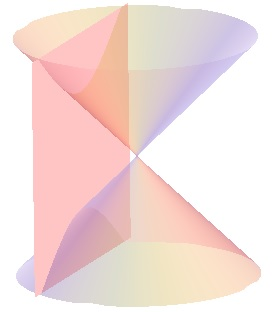
\includegraphics[width=\textwidth]{img/iperbole2.jpg}
  %    \caption{Generazione di un cono a due falde}% 
  %\label{fig:ellissedalcono}
  %    \end{inaccessibleblock}
\end{minipage}  

\subsection{L'iperbole come luogo geometrico}
\label{subsec:iperbole_luogogeometrico}

Usando la sua proprietà di essere un particolare luogo geometrico del 
piano, possiamo definire l'iperbole come:
\begin{definizione}
  Dati nel piano $ \pi $ due punti $ F_{1} $ e $ F_{2} $, detti 
fuochi, si dice iperbole il luogo geometrico I dei punti P di $ \pi $ tali 
che sia costante la differenza delle distanze di P da $F_{1}$ e $F_{2}$ 

\begin{equation}
% I=\{P \in\pi|\overline{PF_{1}}-\overline{PF_{2}}=2a,a\in R_{+}^{0}\}
  E=\{P \in\pi \sand \abs{PF_{1}-PF_{2}} = 2a,~2a \geq 0\}
\end{equation}
\end{definizione}

% \begin{figure}[h]
  %\hspace{12pt}
  \begin{minipage}[c]{.75\textwidth}
Leggiamo la formulazione della definizione. La differenza delle distanze 
tra due punti definiti chiamati fuochi e un generico punto P dell'iperbole 
risulta fissata e pari, sempre, a 2a, qualsiasi sia il punto dell'iperbole. 
Questa lunghezza, 2a, è associata ad un numero reale non negativo.
I diversi punti P appartenenti al luogo geometrico dovranno dunque 
mantenere costante la differenza tra le lunghezze dei segmenti 
$\overline{PF_{1}}$ e $\overline{PF_{2}}$ come indicato nella figura a 
fianco:
  \end{minipage}
  \hspace{.5cm}
  \begin{minipage}[c]{.20\textwidth}
    %    \begin{inaccessibleblock}[Cono a due falde tagliato da un piano
    %      che forma un'ellisse.]
    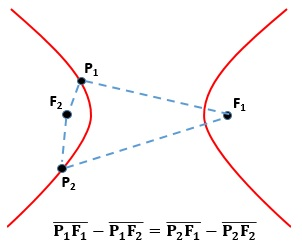
\includegraphics[width=\textwidth]{img/iperbol1.jpg}
%     \caption{L'iperbole come luogo geometrico.}
    %\label{fig:ellissedalcono}
    %    \end{inaccessibleblock}
  \end{minipage}
% \end{figure}

% \begin{figure}[h]
  %\hspace{12pt}
  \begin{minipage}[c]{.2\textwidth}
    %    \begin{inaccessibleblock}[Cono a due falde tagliato da un piano
    %      che forma un'ellisse.]
    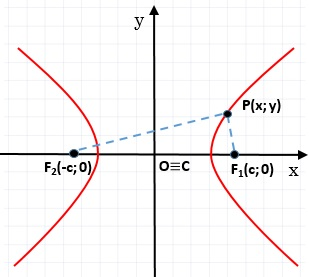
\includegraphics[width=\textwidth]{img/iperbol2.jpg}
%     \caption{i fuochi dell'iperbole.}
    %\label{fig:ellissedalcono}
    %    \end{inaccessibleblock}
  \end{minipage}
  \hspace{.5cm}
  \begin{minipage}[c]{.75\textwidth}
Cerchiamo ora di determinare l'equazione algebrica associata a 
questa curva.
Consideriamo i due fuochi $ F_{1}(-c;~0)$ e $ F_{2}(0;~c)$ sull'asse 
delle X e chiamiamo il punto medio del segmento $\overline{F_{1}F_{2}}$ 
centro dell'iperbole con tale segmento $\overline{F_{1}F_{2}}$  detto 
distanza focale, pari a $\overline{F_{1}F_{2}} =2c$, mentre 2a è la 
distanza che deve rimanere costante per verificare il luogo geometrico in 
oggetto tale che sia valido: 
$\left|\overline{PF_{1}}-\overline{PF_{2}}\right|=2a$. 
  Utilizzando la formula per trovare la lunghezza di un segmento 
possiamo riscrivere il precedente modulo come:
    $\left|\sqrt{(x-c)^{2}+y^{2}} -\sqrt{(x+c)^{2}+y^{2}}\right|=2a$.
  \end{minipage}
% \end{figure}

Sviluppando i calcoli come si è fatto per l'ellisse, con alcuni passaggi 
algebrici si ottiene l'espressione:

$\left( c^{2} -a^{2}\right) x^{2}+a^{2}y^{2}=a^{2}\left(c^{2}-a^{2}\right)$

Ora con la sostituzione $ c^{2}-a^{2}=b^{2} $ 
otteniamo la più semplice: $b^{2}x^{2}-a^{2}y^{2}=a^{2}b^{2}$  
che dividendo entrambi i membri per $a^{2}b^{2}$ assume l'espressione:
\begin{equation}
\dfrac{x^{2}}{a^{2}}-\dfrac{y^{2}}{b^{2}}=1
\end{equation}
detta equazione canonica dell'iperbole avente i fuochi sull'asse X.

\subsection{Le caratteristiche dell'iperbole}
\label{subsec:iperbole_caratteristiche}

\begin{description}
\item [Intersezioni con gli assi]: il grafico dell'iperbole, 
come abbiamo visto, interseca solo l'asse delle X in due punti $ A_{1} 
(a;~0)$ e $ A_{2}(-a;~0)$ le cui coordinate possono facilmente essere 
trovate risolvendo il sistema:

\centerline{$\begin{cases}  \dfrac{x^{2}}{a^{2}}-\dfrac{y^{2}}{b^{2}}=1   
\\ y =0  
  \end{cases} \Rightarrow \begin{cases}  x=a  \\ y=0
  \end{cases}$}

Tali punti vengono detti vertici reali, l'asse che li congiunge, che 
coincide con X, è detto asse trasverso, mentre l'asse Y dove non vi sono 
intersezioni con l'iperbole viene detto asse non trasverso.\\
\item [Simmetrie dell'iperbole]: dato che nell'equazione canonica sia 
la variabile x che la variabile y appaiono di secondo grado se P (x, y) è 
un generico punto dell'iperbole anche i punti $ P_{1}(-x;~y)$,     $ 
P_{2}(-x;~-y)$ e $ P_{3}(x;~-y)$ appartengono all'iperbole e possiamo 
affermare dunque che l'iperbole è una curva simmetrica rispetto all'asse X, 
rispetto all'asse Y e rispetto all'origine.\\
\item [Vertici non reali, asintoti e la costruzione dell'iperbole]:
 abbiamo appena mostrato che il parametro a ci dà le ascisse dei  punti di 
intersezione dell'iperbole con l'asse delle X, possiamo affermare qualcosa 
di simile per il parametro b? Sicuramente non nella stessa forma, in quanto 
l'iperbole non ha intersezioni con l'asse Y. 

% \begin{figure}[h]
  %\hspace{12pt}
  \begin{minipage}[c]{.65\textwidth}
  Tuttavia risulta comodo definire, parallelamente ai due vertici 
reali, altri due vertici, stavolta non reali sull'asse delle Y: i punti $ 
B_{1} (0; b)$ e $ B_{2} (0; -b)$. Non reali in quanto non identificano una 
intersezione reale.\\ Costruiamo ora un rettangolo di lati 2a e 2b con i 
punti $ A_{1} $, $ A_{2} $, $ B_{1} $ e $ B_{2} $, punti medi di tali lati: 
il segmento che congiunge l'origine ad uno dei vertici risulta lungo c, da 
quanto visto nella determinazione dell'equazione dell'iperbole infatti $ 
c^{2} = a^{2} + b^{2} $.
  \end{minipage}
  \hspace{.5cm}
  \begin{minipage}[c]{.3\textwidth}
    %    \begin{inaccessibleblock}[Cono a due falde tagliato da un piano
    %      che forma un'ellisse.]
    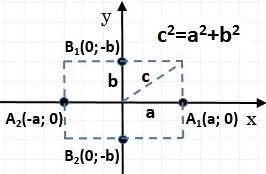
\includegraphics[width=\textwidth]{img/rettangolo.jpg}
%     \caption{Relazione tra i parametri dell' iperbole.}
    %\label{fig:ellissedalcono}
    %    \end{inaccessibleblock}
  \end{minipage}
% \end{figure}

Cerchiamo di capire la relazione tra il rettangolo appena determinato e 
l'iperbole.

% \begin{figure}[h]
  %\hspace{12pt}
  \begin{minipage}[c]{.65\textwidth}
    L'iperbole tocca il rettangolo $A_{1} A_{2} B_{1} B_{2}$ 
soltanto nei vertici reali $A_{1}$ e $A_{2}$ e si sviluppa 
illimitatamente all'interno delle due parti di piano delimitate da due 
rette, chiamate asintoti. Gli asintoti non sono altro che la prosecuzione 
delle diagonali del rettangolo ed hanno come coefficiente angolare m=$ \pm 
$b/a. Gli stessi asintoti forniscono una sorta di limite ne valicabile ne 
raggiungibile da parte dell'iperbole. Le equazioni di queste rette, 
passanti per l'origine sono $y = \dfrac{b}{a} $ e $y =- \dfrac{b}{a}$.
  \end{minipage}
  \hspace{.2cm}
  \begin{minipage}[c]{.3\textwidth}
    %    \begin{inaccessibleblock}[Cono a due falde tagliato da un piano
    %      che forma un'ellisse.]
    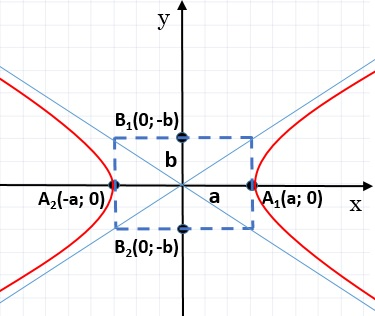
\includegraphics[width=\textwidth]{img/asintoti.jpg}
%     \caption{il rettangolo caratteristico dell'iperbole.}
    %\label{fig:ellissedalcono}
    %    \end{inaccessibleblock}
  \end{minipage}
% \end{figure}

Notiamo infine che possiamo esprimere le coordinate dei fuochi in funzione 
di a e b come: $ F_{1}(\sqrt{a^{2}+b^{2}}, 0) $, $ 
F_{2}(-\sqrt{a^{2}+b^{2}}, 0) $
\item [Eccentricità] Analogamente a 
quanto visto per l'ellisse definiamo l'eccentricità di un iperbole quel 
valore pari al rapporto tra distanza focale e lunghezza dell'asse trasverso:
\begin{equation}
e=\dfrac{distanza \quad focale}{lunghezza \quad asse\quad 
trasverso}=\dfrac{2c}{2a}=\dfrac{c}{a}=\dfrac{\sqrt{a^{2}+b^{2}}}{a}
\end{equation}
poiché dalla precedente formula c>a osserviamo che e>1.
Per comprendere il significato geometrico dell'eccentricità e notare come 
al suo variare cambi il grafico dell'iperbole, studiamo come cambia 
l'eccentricità al variare di b tenendo fissa a, con i seguenti esempi:
\begin{figure}[htbp]
  \centering
  %    \begin{inaccessibleblock}[Cono a due falde tagliato da un piano
  %      che forma un'ellisse.]
  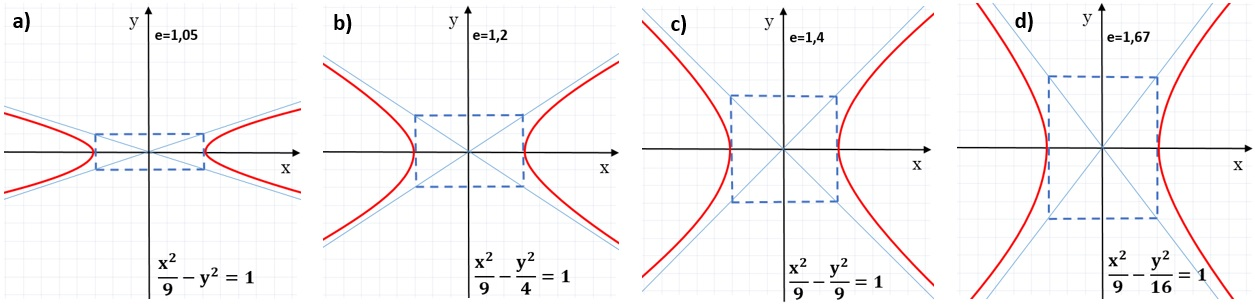
\includegraphics[width=\textwidth]{img/4iperboli.jpg}
    \caption{Eccentricità dell'iperbole al variare del 
parametro b.}%
  %\label{fig:ellissedalcono}
  %    \end{inaccessibleblock}
\end{figure}
\end{description}

\subsection{L'iperbole con i fuochi sull'asse Y}

Se i fuochi, al contrario di quanto visto finora, giacciono sull'asse Y e 
hanno coordinate $ F_{1} (0;~-c)$ e $ F_{2} (0;~c)$ prende forma una nuova 
tipologia di iperbole che invece di svilupparsi a sinistra e a destra 
dell'origine si sviluppa sopra e sotto di tale punto.
Con ragionamenti molto simili ai precedenti partendo stavolta dalla: 
$\left|\overline{PF_{1}}-\overline{PF_{2}}\right|=2b$ riusciamo a 
determinare l'equazione canonica di questo tipo di iperbole che è: 
\begin{equation}
\dfrac{x^{2}}{a^{2}}-\dfrac{y^{2}}{b^{2}}=-1
\end{equation}
Si può poi verificare che:
\begin{itemize} [noitemsep]
  \item l'iperbole è simmetrica rispetto all'origine e agli assi 
cartesiani ;
  \item l'asse Y è l'asse trasverso e su di esso giacciono i vertici 
reali $ B_{1} (0;~b)$ e $ B_{2} (0;~-b)$;
  \item l'asse X è l'asse non trasverso dove giacciono i vertici non 
reali $ A_{1} (a;~0)$ e $ A_{2} (-a;~0)$;
  \item le rette di equazione y=$ \dfrac{b}{a} $ x  e   
$y=-\dfrac{b}{a} x$ sono gli asintoti dell'iperbole ;
  \item è definita l'eccentricità 
$e=\dfrac{c}{b}=\dfrac{\sqrt{b^{2}+a^{2}}}{b} $
\end{itemize}

\subsection{Condizioni per determinare l'equazione dell'iperbole}

Similmente a quanto visto per l'ellisse, essendo anche l'iperbole 
determinata da due parametri, a e b, serviranno solo due condizioni per 
trovarne l'equazione completa e caratterizzante.
Le coppie di informazioni che insieme consentono di determinare un'iperbole 
sono:
\begin{itemize} [noitemsep]
\item la conoscenza di due punti dell'iperbole, non simmetrici rispetto 
agli assi o rispetto all'origine;
\item la conoscenza di un punto e un fuoco (o un vertice);
\item sono noti un fuoco e un vertice;
\item la conoscenza dell'eccentricità e di un fuoco, o di un vertice, o di 
un punto dell'iperbole;
\item la conoscenza di un asintoto e di un fuoco, o un vertice o un punto 
dell'iperbole.
\end{itemize}

\subsection{L'iperbole equilatera e la funzione omografica}
\label{subsec:iperbole_omografica}

Se le lunghezze dei semiassi trasverso e non trasverso sono uguali, a=b, 
l'equazione dell'iperbole diventa: 
$ \dfrac{x^{2}}{a^{2}}-\dfrac{y^{2}}{a^{2}}=1$,   equivalente a   $ 
x^{2}-y^{2} $=$ a^{2} $. 
Tale forma di iperbole, con un solo parametro è detta 
\emph{iperbole equilatera riferita ai propri assi}. 
In questo caso gli altri elementi che caratterizzano l'iperbole diventano:

\vspace{12pt}
% \begin{figure}[h]
  %\hspace{12pt}
  \noindent\begin{minipage}[c]{.65\textwidth}
  \begin{itemize} [noitemsep]
    \item gli asintoti sono $y=x$ e $y=-x$ cioè le bisettrici dei quadranti;
    \item la semidistanza focale c diventa c=a$ \sqrt{2} $;
    \item l'eccentricità è $e = \dfrac{\sqrt{a^{2}+a^{2}}}{a}=\sqrt{2} $
    \item i fuochi sono $ F_{1} \left(a \sqrt{2};~0\right)$ e 
                        $ F_{2}\left(-a \sqrt{2};~0\right)$
    \item i vertici reali sono $ A_{1}(a;~0)$ e $A_{2}(-a;~0)$  
    \item il rettangolo che prima caratterizzava l'iperbole diventa ora 
          un quadrato di lato 2a. 
  \end{itemize}    
  \end{minipage}
  \hfill
  \begin{minipage}[c]{.3\textwidth}
    %    \begin{inaccessibleblock}[Cono a due falde tagliato da un piano
    %      che forma un'ellisse.]
    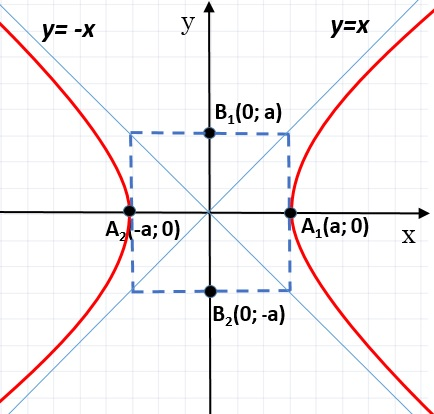
\includegraphics[height=4cm, width=4cm,]{img/equilatera.jpg}
%     \caption{L'iperbole equilatera.}
    %\label{fig:ellissedalcono}
    %    \end{inaccessibleblock}
  \end{minipage}
% \end{figure}

\vspace{12pt}
Nel caso simmetrico in cui i fuochi appartengono all'asse Y 
l'equazione diventa:\\
$ x^{2} - y^{2} =- a^{2} $, con i fuochi 
$ F_{1} \left(0; a \sqrt{2}\right)$, $ F_{2} \left(0;~-a \sqrt{2}\right)$ 
e vertici reali $ B_{1} (0; a)$,$ B_{2} (0; -a)$.
Se ruotiamo di $45\grado$ l'iperbole equilatera riferita ai propri 
assi otteniamo una nuova iperbole che ha come asintoti gli assi cartesiani 
e come assi di simmetria le bisettrici dei quadranti, chiamiamo questo tipo 
di iperbole: \emph{iperbole equilatera riferita ai propri asintoti}.

Si può dimostrare che l'equazione di tale iperbole si può scrivere nella 
forma: 
\begin{equation}
x\cdot y=k \hspace{1cm} con \hspace{0.2cm}k \neq 0
\end{equation}
nel dettaglio a seconda del segno di k abbiamo: 
\begin{figure}[!h]
  \centering
  %    \begin{inaccessibleblock}[Cono a due falde tagliato da un piano
  %      che forma un'ellisse.]
  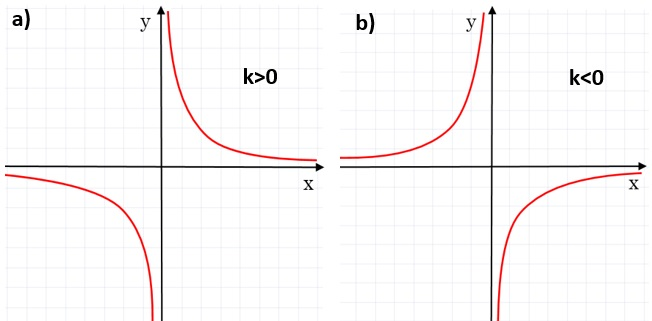
\includegraphics[height=6cm, width=10.5cm]{img/equilatera2.jpg}
  \caption{Iperbole equilatera con k>0 e k<0.}
  %\label{fig:ellissedalcono}
  %    \end{inaccessibleblock}
\end{figure}

Notiamo che l'equazione xy=k non è altro che l'espressione della 
proporzionalità inversa tra due grandezze che mantengono costante il loro 
prodotto e k è la loro costante di proporzionalità. Soffermiamoci sulla 
figura~\(10a\), i vertici di questa iperbole, utili per disegnarla, sono dati 
dall'intersezione dell'iperbole con la bisettrice del primo e terzo 
quadrante. Mettendo a sistema \(xy=k\) e \(x=y\) otteniamo che i vertici sono 
$A_{1} \left( \sqrt{k},~\sqrt{k} \right)$ e 
$A_{2} \left(- \sqrt{k},~-\sqrt{k} \right)$.

\vspace{6pt}
\noindent\begin{minipage}{.6\textwidth}
Vi è un'altra importante scrittura che rappresenta un'iperbole 
equilatera, una funzione matematica che viene rappresentata nel piano come 
un'iperbole traslata rispetto all'origine.
Tale funzione, detta \emph{funzione omografica} è data dalla curva 
di equazione:
\begin{equation}
y= \dfrac{ax+b}{cx+d}
\end{equation}

con \(a,b,c,d\in \R,\quad c \neq 0 \quad \text{e} \quad ad-bc \neq 0\)

\vspace{6pt}
La funzione appena trovata è un'iperbole equilatera che ha come asintoti le 
rette $y= \dfrac{a}{c} $ e $x=-\dfrac{d}{c}$ e come centro di simmetria il 
punto \(C \punto{-\dfrac{d}{c}}{\dfrac{a}{c}}\).
\end{minipage}
\hfill
\begin{minipage}{.35\textwidth}
% \begin{figure}[!htbp]
  \centering
  %    \begin{inaccessibleblock}[Cono a due falde tagliato da un piano
  %      che forma un'ellisse.]
  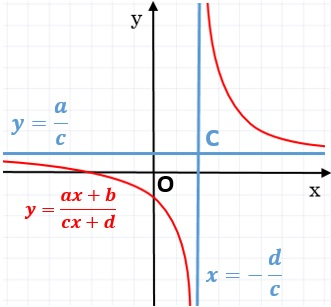
\includegraphics[height=5cm, width=5cm]{img/omografica.jpg}
%   \caption{Funzione omografica.}%
  %\label{fig:ellissedalcono}
  %    \end{inaccessibleblock}
% \end{figure}
\end{minipage}

\vspace{6pt}
Cerchiamo di capire meglio il significato delle due condizioni 
precedentemente poste nell'equazione della funzione omografica:

\begin{itemize} [noitemsep]
  \item se c= 0 otteniamo $y= \dfrac{ax+b}{d} $ cioè $y= 
\dfrac{ax}{d} + \dfrac{b}{d} $, che rappresenta una semplice retta;
  \item se $ad-bc=0$, cioè $ \dfrac{d}{c} = \dfrac{b}{a} $, 
l'equazione si può scrivere nella forma:
y= $\dfrac{ax+b}{cx+d}=  \dfrac{a\left(x+ \frac{b}{a} \right)}{c\left(x+ 
\frac{d}{c} \right)} $ da cui, per $x \neq -\dfrac{d}{c} $, abbiamo y=$ 
\dfrac{a}{c} $; cioè, se $ad-bc=0$ otteniamo una retta di equazione y=a/c 
definita per tutte le x escluso il valore $x=-d/c$.  
\end{itemize}

\begin{esempio}
~

% \begin{figure}[h]
  %\hspace{12pt}
  \begin{minipage}[c]{.6\textwidth}
    Data l'iperbole equilatera $ x^{2} - y^{2} =6$, determina i 
vertici i fuochi e c, infine disegnala.\\
    Poiché $a= \sqrt{6} $, i vertici risultano $ A_{1} 
\left(\sqrt{6};~ 0\right)$ e $ A_{2} \left(-\sqrt{6};~ 0\right)$ e $c= 
\sqrt{6}  \sqrt{2} = \sqrt{12} =2 \sqrt{3} $. Dalla conoscenza di c 
otteniamo i fuochi $ F_{1} \left(2\sqrt{3};~ 0\right)$ e $ F_{2} 
\left(-2\sqrt{3}; ~0\right)$.
  \end{minipage}
  \hspace{.2cm}
  \begin{minipage}[c]{.35\textwidth}
    %    \begin{inaccessibleblock}[Cono a due falde tagliato da un piano
    %      che forma un'ellisse.]
    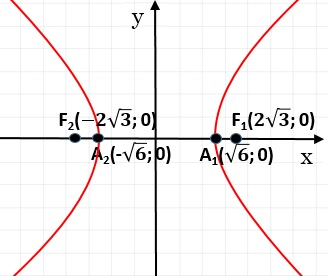
\includegraphics[width=\textwidth]{img/equilatera1.jpg}
    %\caption{Generazione di un'ellisse da un cono a due falde}
    %\label{fig:ellissedalcono}
    %    \end{inaccessibleblock}
  \end{minipage}
% \end{figure}
\end{esempio}

\begin{esempio}
~

% \begin{figure}[h]
  %\hspace{12pt}
  \begin{minipage}[c]{.6\textwidth}
    Data l'iperbole equilatera $xy=8$, determina i suoi vertici 
e disegnala.\\ Si tratta di un'iperbole equilatera riferita ai propri 
asintoti e poiché k> 0 si trova nel primo e nel terzo quadrante. I vertici 
sono: $ A_{1} \left(2\sqrt{2}; 2\sqrt{2}\right)$ e $ A_{2} 
\left(-2\sqrt{2}; -2\sqrt{2}\right)$
  \end{minipage}
  \hspace{.2cm}
  \begin{minipage}[c]{.35\textwidth}
    %    \begin{inaccessibleblock}[Cono a due falde tagliato da un piano
    %      che forma un'ellisse.]
    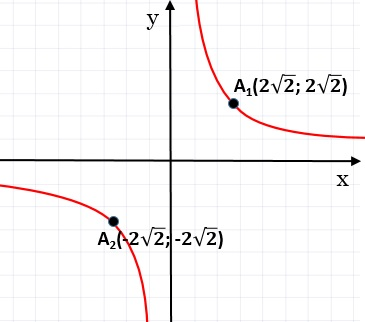
\includegraphics[width=\textwidth]{img/equilatera2a.jpg}
    %\caption{Generazione di un'ellisse da un cono a due falde}
    %\label{fig:ellissedalcono}
    %    \end{inaccessibleblock}
  \end{minipage}
% \end{figure}
\end{esempio}

\begin{esempio} Data la funzione omografica $y= \dfrac{x-3}{x+2}$ 
dopo aver verificato che è un'iperbole , determinane gli 
asintoti e il centro di simmetria. Completa l'esercizio facendo il disegno 
della funzione.

Per verificare se si tratta di un iperbole constatiamo che 
$c=1$, quindi $c \neq 0$ e poi calcoliamo $ad-bc$. Se questa espressione è 
diversa da~0 la funzione omografica rappresenta una iperbole: $ad-bc=5$. 
Possiamo ora determinare gli asintoti, quello verticale è 
$x=- \dfrac{d}{c} =-2$ e quello orizzontale è $y= \dfrac{a}{c} =1$; 
il centro di simmetria è $C(-2; ~1)$.

% \begin{figure}[h]
  %\hspace{12pt}
  \begin{minipage}[c]{.65\textwidth}
     Per disegnare la funzione dobbiamo avere i riferimenti dei 
punti in cui il grafico interseca gli assi, per trovare quella con l'asse X 
basta risolvere il sistema tra la funzione e x=0, per determinare quella 
con Y basta risolvere il sistema tra l'equazione e y=0. i due punti cercati 
sono $ P_{1}  \left(0;~ - \dfrac{3}{2} \right)$ e $ P_{2} =(3;~0)$.
  \end{minipage}
  \hfill
  \begin{minipage}[c]{.25\textwidth}
    %    \begin{inaccessibleblock}[Cono a due falde tagliato da un piano
    %      che forma un'ellisse.]
    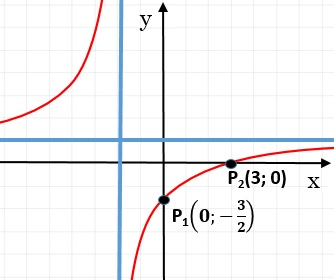
\includegraphics[width=\textwidth]{img/equilatera2b.jpg}
    %\caption{Generazione di un'ellisse da un cono a due falde}
    %\label{fig:ellissedalcono}
    %    \end{inaccessibleblock}
  \end{minipage}
% \end{figure}
\end{esempio}


  


